\section{Oblique impact with a fixed surface}
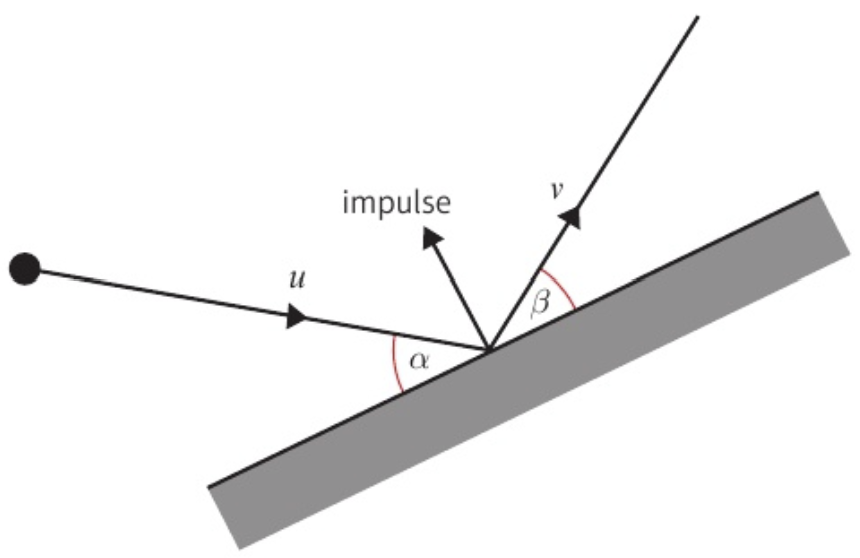
\includegraphics[width=0.3\textwidth]{obliqueimpact}
\begin{itemize}
    \item The component of the velocity of the sphere parallel to the surface is unchanged: $v\cos\beta = u\cos\alpha$
    \item The component of the velocity of the sphere perpendicular to the surface can be found with Newton's law of restitution: $v\sin\beta = eu\sin\alpha$
    \item Hence $\tan\beta = e\tan\alpha$, since $0 \leq e \leq 1$, $\beta \leq \alpha$
    \item $\text{Loss of kinetic energy}=\dfrac{1}{2}mu^2-\dfrac{1}{2}mv^2$
\end{itemize}
\section{Oblique impact of smooth spheres}
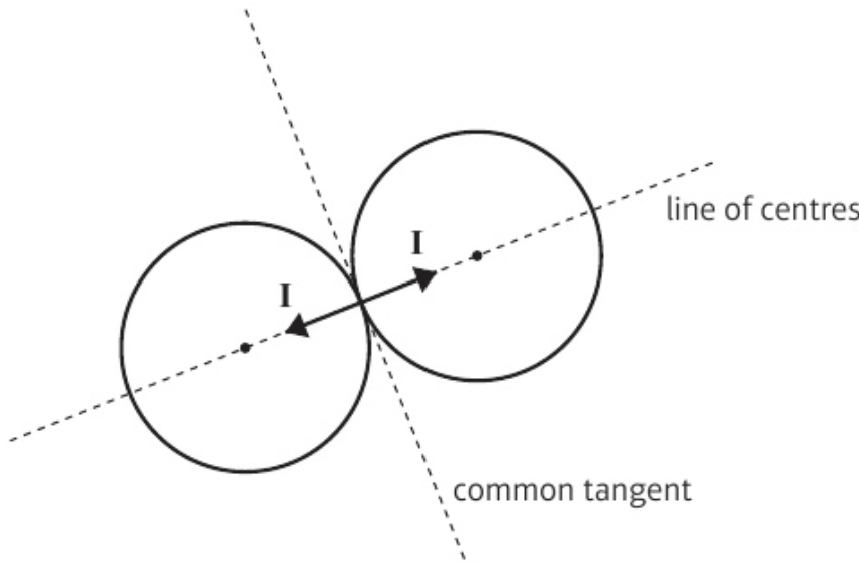
\includegraphics[width=0.3\textwidth]{oblique_2_balls}
\begin{itemize}
    \item Impulse affecting each sphere acts along the line of centres
    \item The components of the velocities of the spheres \textbf{perpendicular}  to the line of centres are unchanged in the impact
    \item The principle of conservation of momentum and Newton's law of restitution applies \textbf{parallel} to the line of centres
\end{itemize}